\documentclass{optica-article}
\usepackage{xcolor} 
\definecolor{darkred}{HTML}{BA1A1A}
\definecolor{extralightgray}{HTML}{F5F5F5}

\journal{opticajournal} % for journals or Optica Open

\articletype{Research Article}

\usepackage{lineno}
\usepackage{todonotes}
\linenumbers % Turn off line numbering for Optica Open preprint submissions.

\begin{document}

\title{Data Recovery and Pulse Position Modulation with a Photon Number Resolving SNSPD}

\author{Author One,\authormark{1} Author Two,\authormark{2,*} and Author Three\authormark{2,3}}

\address{\authormark{1}Peer Review, Publications Department, Optica Publishing Group, 2010 Massachusetts Avenue NW, Washington, DC 20036, USA\\
\authormark{2}Publications Department, Optica Publishing Group, 2010 Massachusetts Avenue NW, Washington, DC 20036, USA\\
\authormark{3}Currently with the Department of Electronic Journals, Optica Publishing Group, 2010 Massachusetts Avenue NW, Washington, DC 20036, USA}

\email{\authormark{*}opex@optica.org} %% email address is required; see note below about the corresponding author designation

% use {asbstract*} to suppress the copyright line. Copyright information will be added in production

\begin{abstract*} 
Photon number resolution is an emerging capability of advanced Superconducting Nanowire Single Photon Detectors. If leveraged to it's full potential, PNR capability can have a profound impact on the usefulness of SNSPDs is certain quantum applications including linear optical quantum computing, quantum networks, and quantum sensing. Discrimination of not just the number of photons in an optical pulse but also pulse arrival time with high accuracy is an open problem, complicated by the nuanced way in which these two degrees of freedom are intertwined in the response function of these detectors. In this work we test a differential readout SNSPD in a Pulse Position Modulation experiment whereby data is sent in the arrival time of optical pulses derived from a 20~GHz optical clock. We show the detector is capable of discriminating the arrival time of photons to 50~ps wide bins with high accuracy while simultaneously providing photon number information about the impinging optical pulses. We find that cluster analysis and gaussian mixture models are useful for extracting precise measurements of pulse arrival time and photon number.
\end{abstract*}

%%%%%%%%%%%%%%%%%%%%%%%%%%  body  %%%%%%%%%%%%%%%%%%%%%%%%%%
\hypertarget{introduction}{%
\section{Introduction}\label{introduction}}

\textcolor{red}{ The following is very rough, taken from years ago when I first started writing the manuscript }

This study aimed to evaluate the feasibility of transmitting high clock-rate pulse position modulated (PPM) data using a mode-locked laser and receiving it with a low jitter superconducting nanowire single-photon detector (SNSPD). The investigation was driven by recent advancements in NbN SNSPDs, which have achieved a jitter as low as 50 ps at the FW(1/100)M level, enabling the demonstration of PPM with 50 ps slot widths and a 20 GHz clock. The aim was to increase the data rate by a factor of 10, from 2 GHz to 20 GHz, in the next generation of the Deep Space Optical Communication (DSOC) project.

During the course of this study, the focus shifted towards investigating the impact of photon number resolution (PNR) on the low jitter detection of optical pulses. PNR can have an unintended impact on the demonstration of high-rate PPM, and therefore a thorough study of its effects was deemed crucial. A novel PNR cancellation technique was developed and applied to successfully demonstrate high-rate PPM. This technique is considered essential for future low-jitter applications of SNSPDs that exhibit photon-number effects.

This study aimed to evaluate the feasibility of transmitting high clock-rate pulse position modulated (PPM) data using a mode-locked laser and receiving it with a low jitter superconducting nanowire single-photon detector (SNSPD). The investigation was driven by recent advancements in NbN SNSPDs, which have achieved a jitter as low as 50 ps at the FW(1/100)M level, enabling the demonstration of PPM with 50 ps slot widths and a 20 GHz clock. The aim was to increase the data rate by a factor of 10, from 2 GHz to 20 GHz, in the next generation of the Deep Space Optical Communication (DSOC) project.

During the course of this study, the focus shifted towards investigating the impact of photon number resolution (PNR) on the low jitter detection of optical pulses. PNR can have an unintended impact on the demonstration of high-rate PPM, and therefore a thorough study of its effects was deemed crucial. A novel PNR cancellation technique was developed and applied to successfully demonstrate high-rate PPM. This technique is considered essential for future low-jitter applications of SNSPDs that exhibit photon-number effects.

\hypertarget{fig:intro}{%
\begin{figure}
\centering
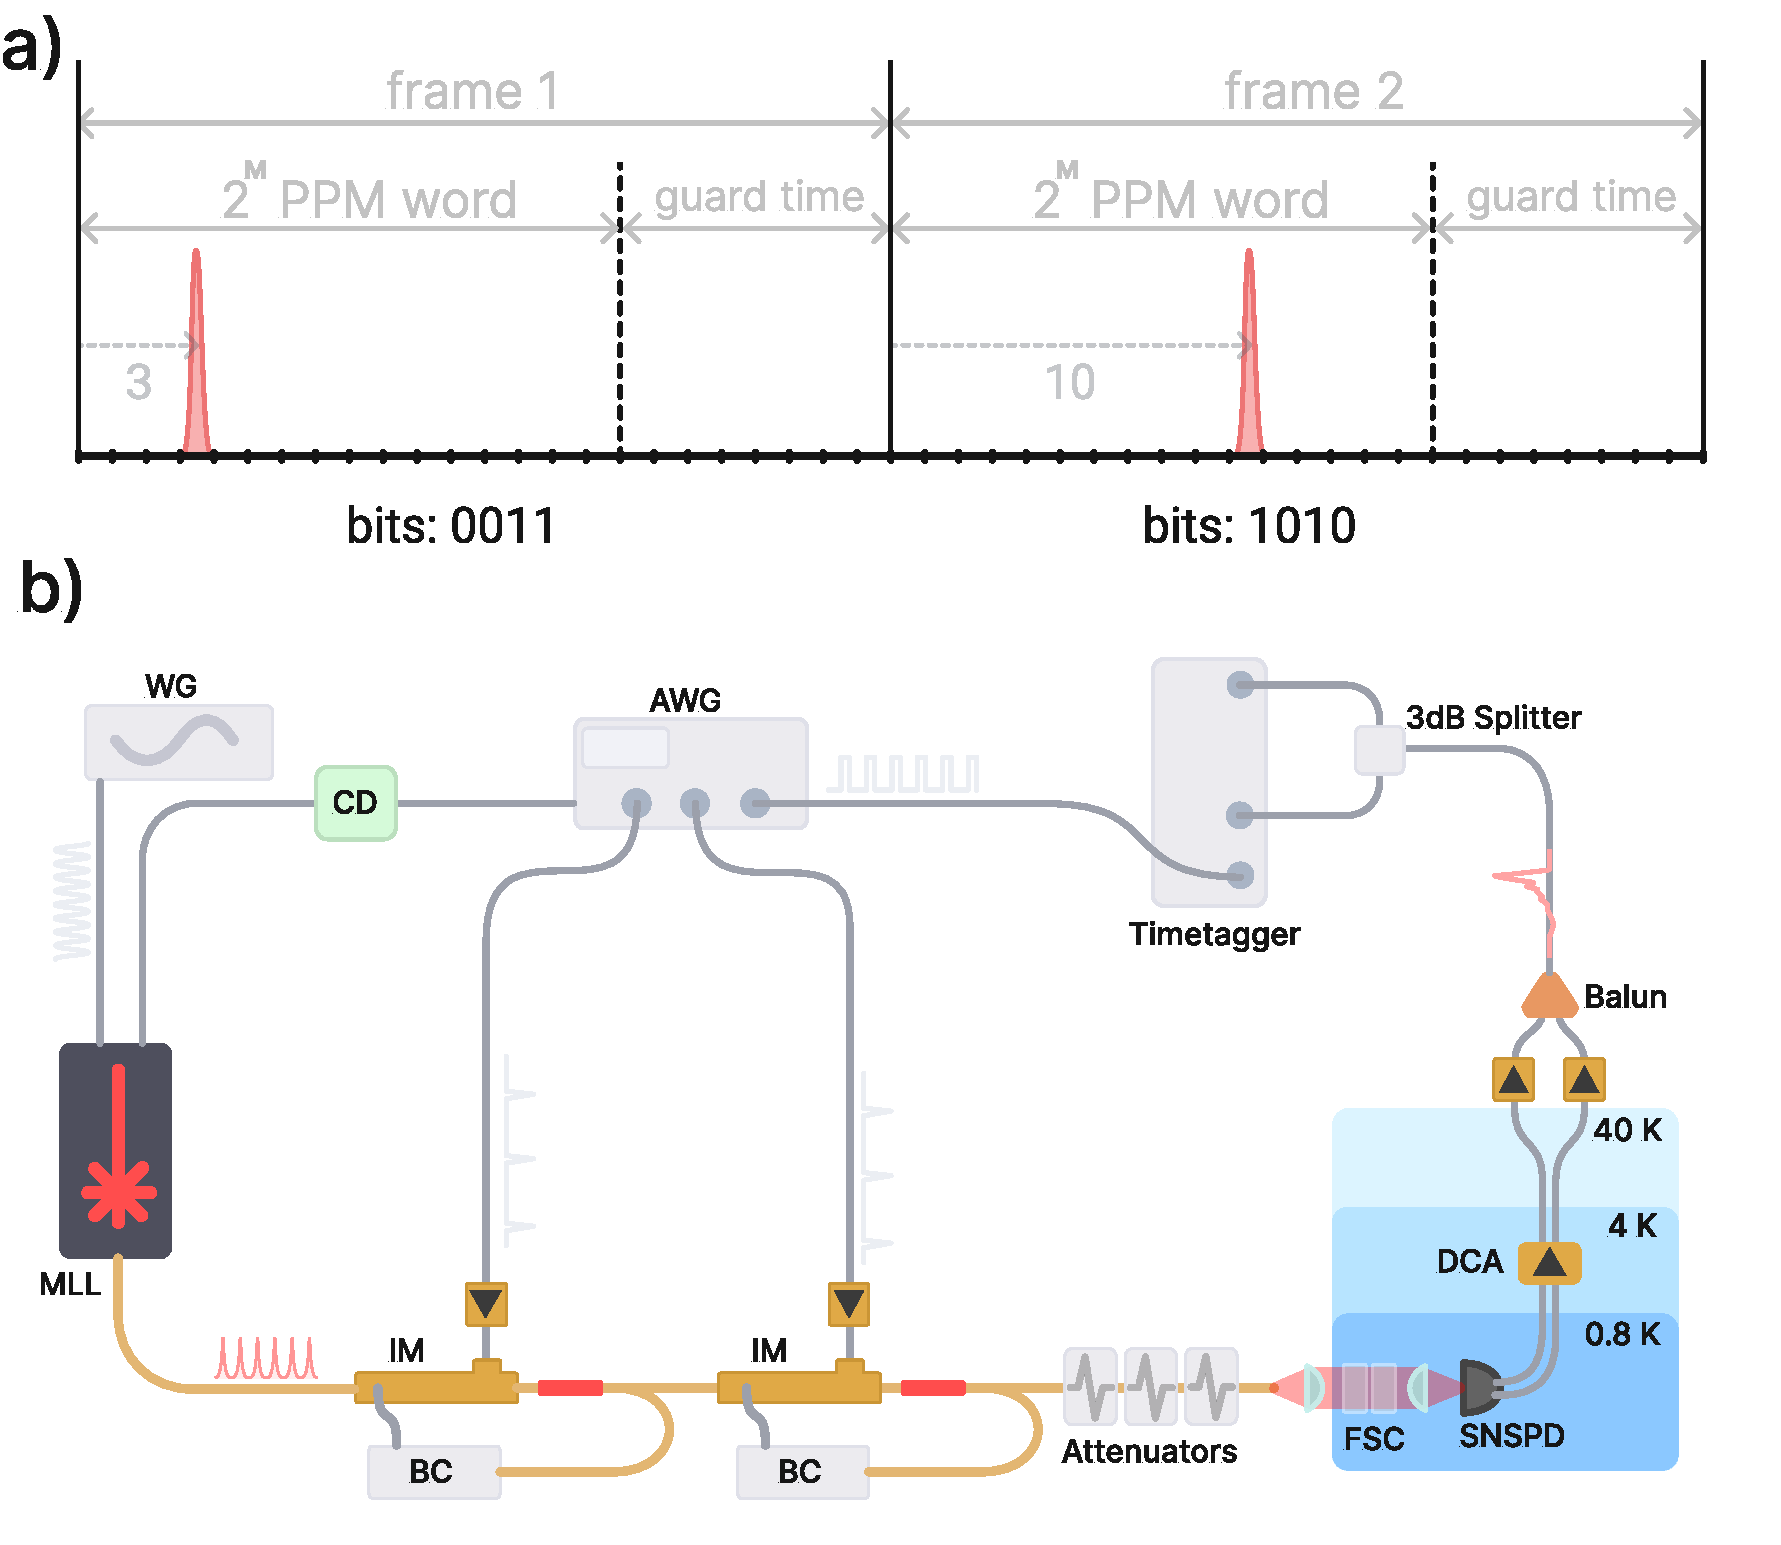
\includegraphics[width=1\textwidth]{./figs_03/fig_intro_light.pdf}
\caption[{PPM modulation and experiment setup}]{\textbf{PPM modulation and experiment setup} a) How bits are transmitted in M=16 PPM modulation. An optical pulse is transmitted with a clock-referenced integer delay which encodes 4 bits of data. b) Diagram of the expiremental setup. WG: wave generator, CD: clock divider board, AWG: Arbitrary Waveform Generator, MLL: Mode Locked Laser (Pritel UAC), IM: Intensity Modulator, BC: Bias Controller, FSC: Free Space Coupling System, DCA: DC Coupled Cryo-amp}
\label{fig:intro}
\end{figure}
}

\hypertarget{pulse-position-modulation-for-deep-space-communication}{%
\subsection{Pulse Position Modulation for Deep Space Communication}\label{pulse-position-modulation-for-deep-space-communication}}

Deep Space Optical Communication has been a growing field of study in recent years, as researchers look for ways to communicate with spacecraft that are far away from Earth. In this article, we will focus on the use of Pulse Position Modulation (PPM) for deep space optical communication.

While other modulation techniques such as quadrature amplitude modulation (QAM) have been used in the past, it has been shown that in the photon-starved regime, PPM is the best approach for sending data. This is because there is not enough light to measure the phase of the signal.

PPM relies on sending one optical pulse carrying M bits of information in one of \(2^M\) possible time slots. For M = 2, this corresponds to sending an early pulse to represent a 0 bit and a late pulse to represent a 1 bit.

The main challenge in deep space optical communication is the high loss and distance that the link must traverse. This limits the communication from the spacecraft, as it is limited by the power available on the spacecraft. This means that the communication protocol is limited by the number of bits that can be sent per unit of energy on the spacecraft, also known as photon information efficiency or bits per photon.

For large M, PPM achieves high photon information efficiency, allowing for the saving of power on the spacecraft and the sending of more information with fewer photons. The existing deep space optical communication project uses M up to \(2^8 = 256\), meaning that 8 bits of data are carried in each optical pulse.

In this project, we aimed to demonstrate even higher photon information efficiency by using M values up to 2048, or 11 bits of data per optical pulse.

While the use of large M values increases photon information efficiency, it also decreases the data rate of the system. This is because the number of time bins needed per optical pulse scales exponentially with the amount of data in each pulse. Therefore, for a given fixed clock rate and time bin duration, the data rate decreases dramatically for higher M values.

Using M values much larger than 11 is unlikely to be practical in future deep space optical communication systems. However, the data rate of these systems can be increased linearly by increasing the clock rate or bin size of the experiment. This is possible with the use of low jitter detection systems or low jitter superconducting nanowire single-photon detectors (SNSPDs).

\hypertarget{detector-figure-of-merit}{%
\section{Detector Figure of Merit}\label{detector-figure-of-merit}}

The work here highlights the application of low jitter single-photon detectors for optical communication, which is impactful for deep-space optical communication as well as classical communication in quantum networks. Although single-photon counting is well estanblished for deep-space optical communication\textasciitilde{}\cite{Laser lunar, DSOC} so far it has not been ulitized in quantum networks, mainly due to the use of SFP modules and DWDMs. However, with the eachievement of high data rates recently achieved with photon-counting classical communication, these approaches can now be seriously considered for quantum networks. The main driver is would be the deduction of optical power in neighbouring DWDM channels, which ultimately lowers the Raman scattered photons into the quantum channel \cite{EraerdsRaman}
\textcolor{red}{Calculate reduction in power from state of the art SFP modules}

To access the applicability of different detectors, here we compare some of the recent near infrared detectors.

A useful figure of merit that includes all of the revelant detector metrics for photon timing was introduced by Bronzi and co-authors \cite{Bronzi2016}

\[FoM_T = \frac{\eta  (1 - P_{ap})\Phi_{-3 \text{dB}}}{J} \sqrt{\frac{A}{D}},\]

where \(\eta\) is the single photon detection efficiency, \(\Phi_{-3 \text{dB}}\) is the photon flux at which the system detection efficiency drops by 3\textasciitilde dB, \(P_{ap}\) is the afterpulsing probability, \(J\) is the detector jitter evaluated as the FWHM, \(T_d\) is the deadtime, \(A\) is the active area and \(D\) is the dark count rate. Here we have defined the maximum photon flux as the 3\textasciitilde dB point, for ease of standardization.

In this work:

\begin{itemize}
\tightlist
\item
  Efficiency = 0.84
\item
  Afterpulsing = 0 \%
\item
  Jitter = 15 ps
\item
  Deadtime = 30 ns \textcolor{red}{measure 3dB flux}
\item
  Area = 330 \(\mu m^2\)
\item
  Dark count rate = 20~Hz
\end{itemize}

\(FoM_T = 7.58 \times 10^{12}\) at 1550 nm.

The deadtime is calculated as the 1/MCR, which is the 3 dB point of the nominal efficiency. This is only a factor of 3.7 less than the state of the art visible Silicon SPADs (peak efficiency at 480\nm) \cite{Gramuglia2022}

In the future, the performance of the optical communication system could be improved by using, high count rate SNSPD arrays. Recently published high-count rate arrays have figures of merit of \textcolor{red}{\(FoM_T\) for Peacoq and Resta2023 results}. This would result in a proportinal increase in the data rate.
\textcolor{red}{\(FoM_T\) for fastest InGaAs/InP gated detector}
These devices are ideal for fiber-based optical communication. In free-space, the active area is especially important, whithout the use of an adaptive optics system.
\textcolor{red}{\(FoM_T\) for DSOC array}

\hypertarget{development-of-a-modulation-source}{%
\subsection{Development of a modulation source}\label{development-of-a-modulation-source}}

The communication signal on a spacecraft is generated by utilizing a Continuous Wave (CW) seed laser that is carved by a fast intensity modulator. The resulting low-power pulsed signal is then amplified by an Erbium Doped Fiber Amplifier (EDFA) to increase its transmission power to Earth. The majority of the power used by the spacecraft for communication scales with the number of optical pulses due to the EDFA.

In our experiment, the 20 GHz repetition rate was limited by the jitter of the Single-Photon Detectors (SNSPDs) that we intended to use. These detectors have a Full Width at Half Maximum (FW(1/100)M) jitter of approximately 50 ps. To ensure that the response function of the entire experiment had jitter of around 50 ps FW(1/100)M, we needed to build a Pulsed Phase Modulation (PPM) source with ultra-short optical pulses.

Carving a CW laser with our system would have introduced excessive timing uncertainty due to the limited ability of even the fastest lithium niobate intensity modulators to carve pulses with widths below 20 ps. The added jitter from modulated CW pulses, combined with the jitter of the detectors, would have exceeded the 20 GHz/50 ps slot width requirement.

Therefore, we chose to carve pulses from a mode-locked laser. This approach allows for extremely short pulses in time, with the modulators responsible for sufficiently reducing any surrounding unwanted pulses. The temporal width of the modulator pulse response must be extremely short and able to modulate from `off' to `on' within a time frame of the order of the 50 ps bin width.

\hypertarget{methods}{%
\section{Methods}\label{methods}}

\hypertarget{results}{%
\section{Results}\label{results}}

results here

\bibliography{references}



\end{document}